\section{数据库概念设计}

\subsection{数据架构概述}

本系统采用分层的数据架构设计,包括数据处理层和规范化数据层两个层次:
\begin{enumerate}
  \item 数据处理层
  \begin{itemize}
    \item 目的:支持数据采集和清洗的ETL过程
    \item 特点:
    \begin{itemize}
      \item 保留原始数据格式,便于追溯和验证
      \item 允许数据冗余,不强制遵循3NF
      \item 支持增量更新和批量处理
    \end{itemize}
    \item 组成:
    \begin{itemize}
      \item 原始数据表:分别存储BOSS直聘和猎聘网的原始爬虫数据
      \item 暂存数据表:存储统一格式和质量检查后的中间数据
    \end{itemize}
  \end{itemize}

  \item 规范化数据层
  \begin{itemize}
    \item 目的:
    \begin{itemize}
      \item 提供高质量的规范化数据
      \item 支持复杂的数据查询和分析
      \item 保证数据一致性
    \end{itemize}
    \item 特点:
    \begin{itemize}
      \item 严格遵循3NF,消除数据冗余
      \item 建立完整的实体关系
      \item 支持事务处理
    \end{itemize}
    \item 组成:
    \begin{itemize}
      \item 基础实体表:包含用户、公司、职位、地址四个核心实体
      \item 关联关系表:维护实体间的多对多关系
      \item 物化视图:预计算常用查询结果,提升查询性能
    \end{itemize}
  \end{itemize}
\end{enumerate}

\begin{figure}[htbp]
  \centering
  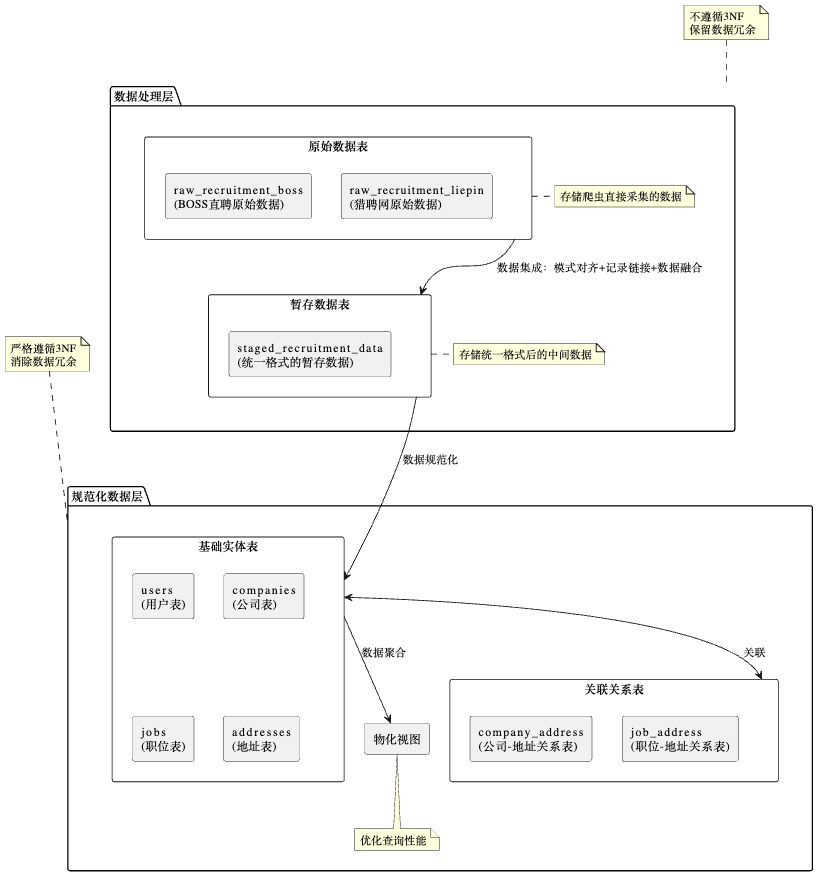
\includegraphics[width=0.8\textwidth]{figures/数据库概念设计.png}
  \caption{系统数据架构图}
  \label{fig:data_architecture}
\end{figure}

如图\ref{fig:data_architecture}所示,系统采用分层架构设计,将数据处理层和规范化数据层进行清晰分离。数据处理层包含BOSS直聘(raw\_recruitment\_boss)和猎聘网(raw\_recruitment\_liepin)的原始数据表,以及用于存储统一格式数据的暂存表(staged\_recruitment\_data),不严格遵循第三范式以支持数据处理和追溯。规范化数据层则严格遵循3NF范式,由用户(users)、公司(companies)、职位(jobs)、地址(addresses)四个基础实体表,以及公司-地址(company\_address)、职位-地址(job\_address)两个关联关系表组成,并通过物化视图(recruitment\_mv)优化查询性能。数据流向是从原始数据经过清洗后存入暂存表,再经规范化处理后存入实体表和关系表,最后通过物化视图提供高效的数据查询服务。


\subsection{实体定义}
规范化数据层包含用户(User)、公司(Company)、职位(Job)和地址(Address)四个核心实体。这些实体严格遵循第三范式设计,消除数据冗余,保证数据一致性。用户实体用于系统访问控制,支持普通用户和管理员两种角色,确保系统安全;公司实体规范化存储招聘企业的基本信息,通过唯一的公司名称避免重复;职位实体以标准化格式记录招聘信息,通过外键关联到发布公司;地址实体则规范化存储地理位置信息,支持地理空间查询。实体之间通过关联关系表维护多对多关系,形成完整且规范的数据模型。表\ref{tab:entity_definition}详细说明了规范化数据层各实体的定义:

\begin{table}[htbp]
  \centering
  \caption{系统实体定义}
  \label{tab:entity_definition}
  \begin{tabular}{|p{0.15\textwidth}|p{0.35\textwidth}|p{0.4\textwidth}|}
    \hline
    \begin{center}\textbf{实体名称}\end{center} & \begin{center}\textbf{主要属性}\end{center} & \begin{center}\textbf{说明}\end{center} \\
    \hline
    \multirow{5}{*}{用户(User)} & 
    \begin{itemize}
      \item 用户ID(主键)
      \item 用户名
      \item 密码
      \item 用户角色
      \item 创建时间
    \end{itemize} & 
    \begin{center}系统用户信息,支持基本的角色权限控制。用户可以分为普通用户和管理员两种角色,用于管理系统访问权限。\end{center} \\
    \hline
    \multirow{6}{*}{公司(Company)} & 
    \begin{itemize}
      \item 公司ID(主键)
      \item 公司名称(唯一)
      \item 所属行业
      \item 公司规模
      \item 创建时间
      \item 更新时间
    \end{itemize} & 
    \begin{center}招聘公司的基本信息。公司名称需要保持唯一性以避免重复,通过所属行业和公司规模等属性可以支持多维度的分析查询。\end{center} \\
    \hline
    \multirow{11}{*}{职位(Job)} & 
    \begin{itemize}
      \item 职位ID(主键)
      \item 职位名称
      \item 职位类型
      \item 薪资范围
      \item 经验要求
      \item 学历要求
      \item 技能要求
      \item 职位福利
      \item 数据来源
      \item 创建时间
      \item 更新时间
    \end{itemize} & 
    \begin{center}职位发布的详细信息。包含职位要求、待遇等完整招聘信息,通过数据来源字段可以追踪数据来源渠道。\end{center} \\
    \hline
    \multirow{6}{*}{地址(Address)} & 
    \begin{itemize}
      \item 地址ID(主键)
      \item 地址文本
      \item 经度
      \item 纬度
      \item 创建时间
      \item 更新时间
    \end{itemize} & 
    \begin{center}公司和职位关联的地理位置信息。通过经纬度坐标支持地理位置检索和距离计算,可用于就近推荐等功能。\end{center} \\
    \hline
  \end{tabular}
\end{table}

图\ref{fig:normalized_data_er}展示了规范化数据层的数据结构设计。该设计严格遵循第三范式(3NF),通过实体表和关系表的合理组织,消除了数据冗余,保证了数据一致性。该E-R图清晰地展示了系统中各实体之间的关联关系,为后续的物理设计和系统实现提供了重要指导。下面是关于图中的实体表User、Company、Job和Address和关系表company\_address、job\_address的详细说明。

\begin{figure}[htbp]
  \centering
  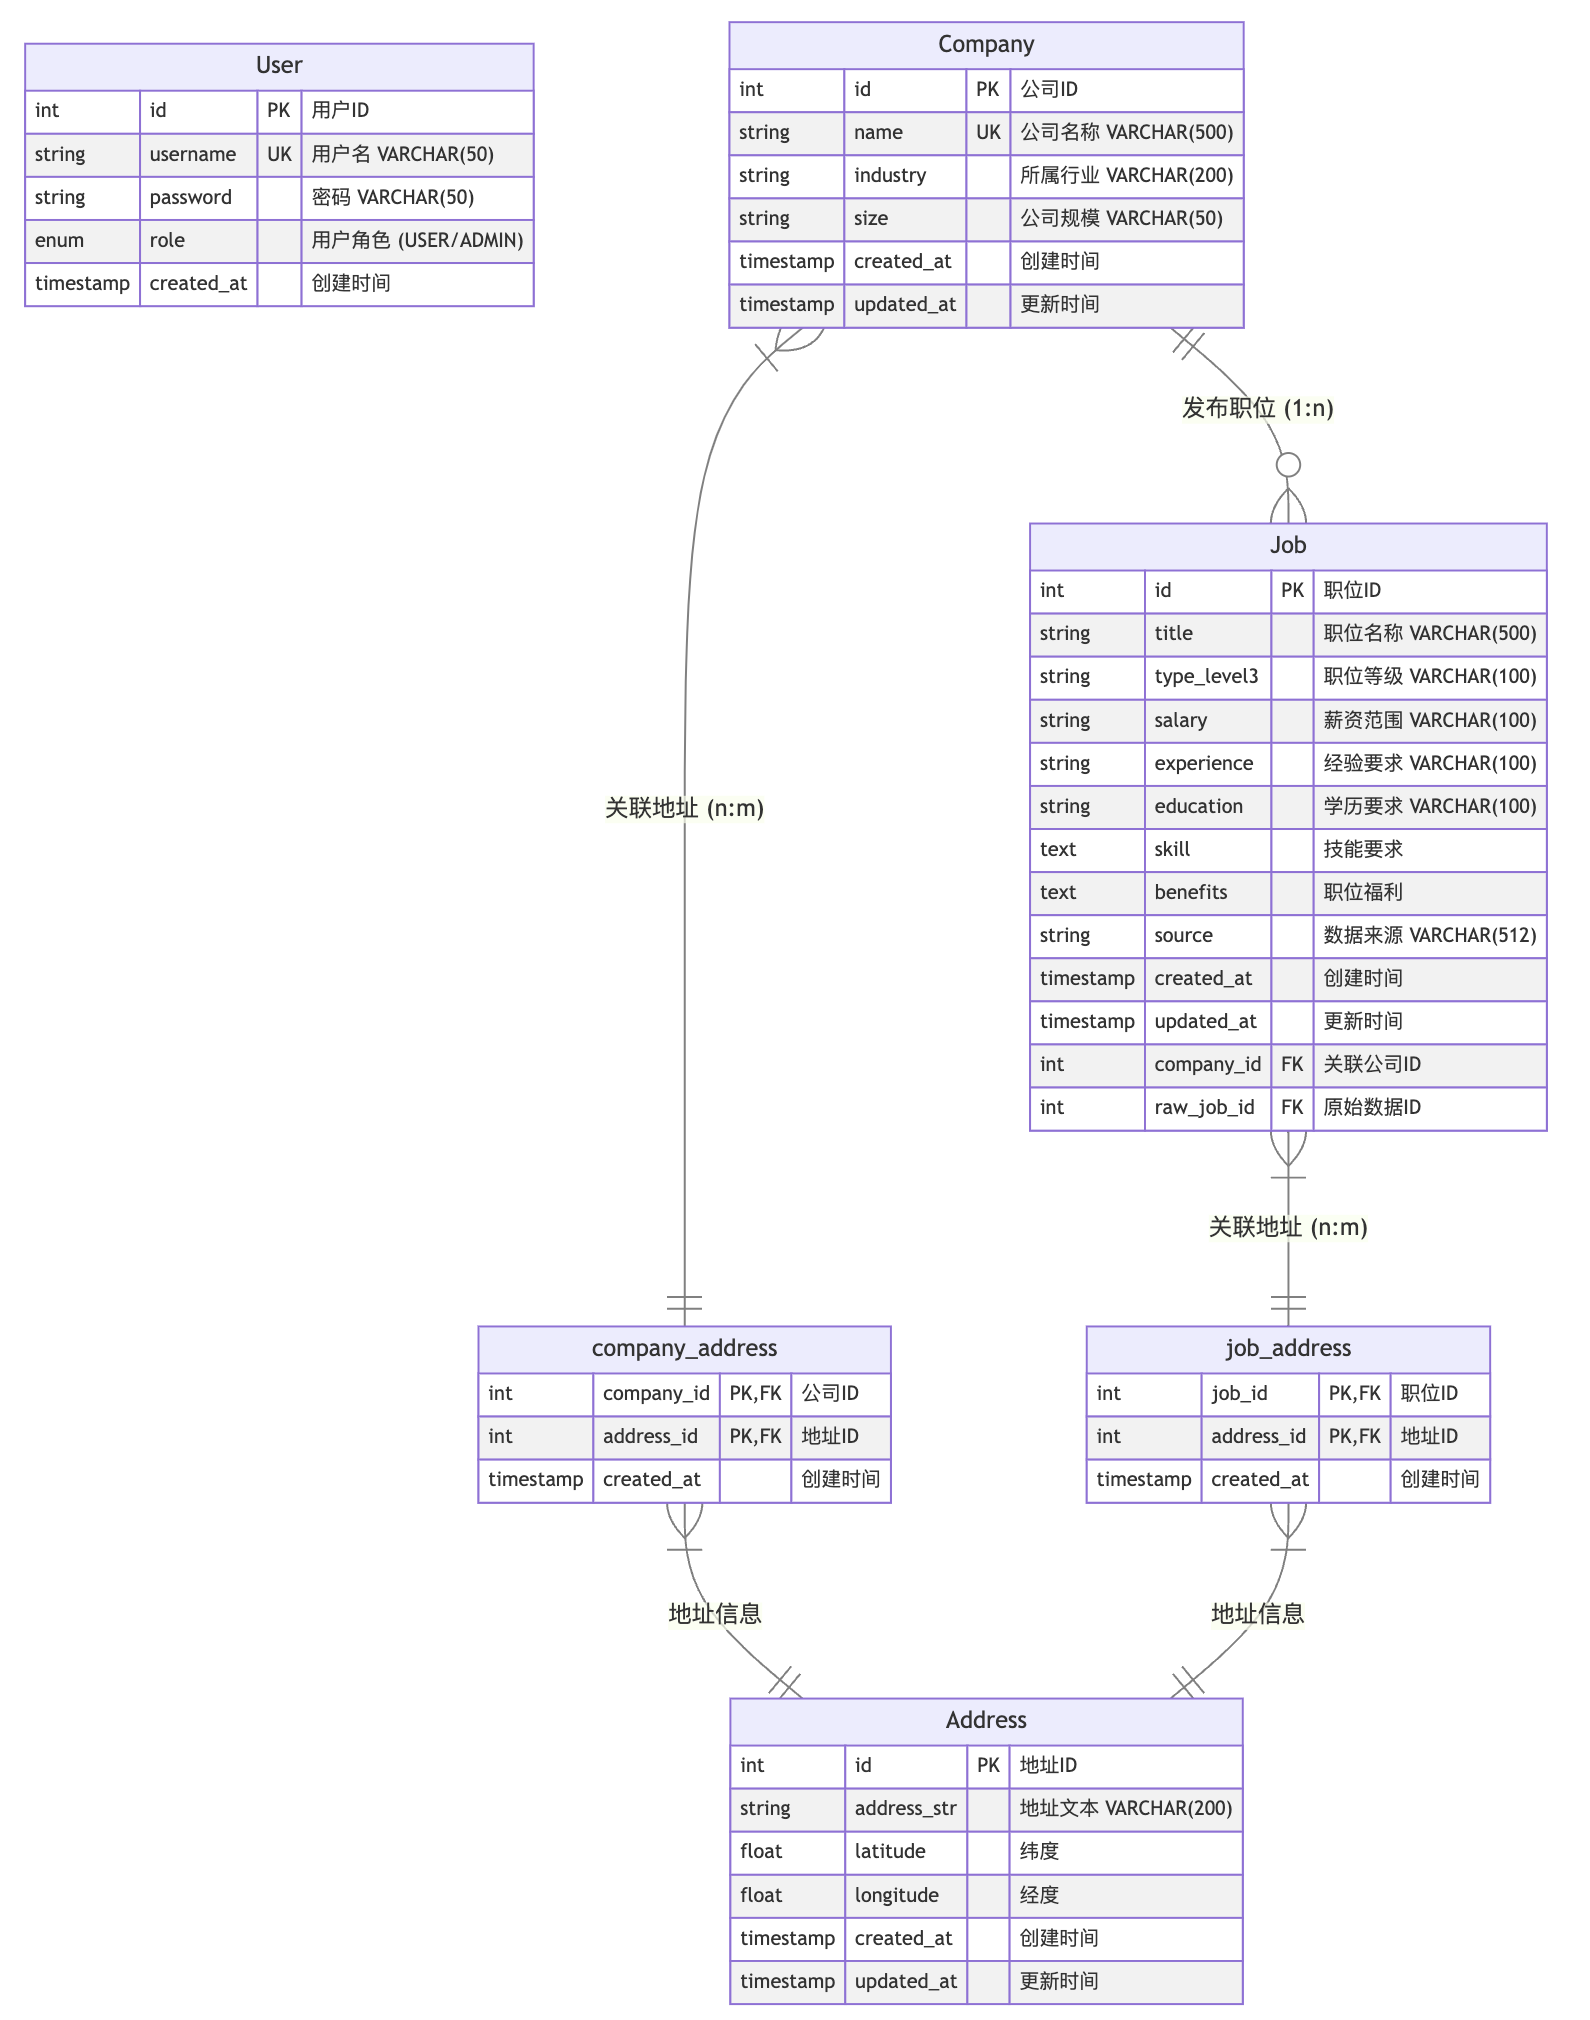
\includegraphics[width=0.8\textwidth]{figures/数据库实体ER图.png}
  \caption{规范化数据层E-R图}
  \label{fig:normalized_data_er}
\end{figure}


\paragraph{核心实体表设计}
系统的数据模型主要由四个基本实体表构成,每个实体表都严格遵循第三范式(3NF)设计原则。用户(User)表作为系统的基础用户管理单元,存储用户的身份认证和授权信息。该表包含用户ID作为主键,用户名设置唯一约束,同时存储密码和用户角色信息。通过角色字段(枚举类型:user/admin)实现基本的权限管理,并在用户名上建立索引(ix\_users\_username)以优化登录查询性能。

公司(Company)表存储招聘公司的核心信息,是职位信息的关联主体。该表以公司ID为主键,公司名称设置唯一约束,同时包含所属行业、公司规模等基本信息字段。为支持多维度的查询需求,表中建立了针对性的复合索引,包括公司名称索引(ix\_companies\_name)、行业规模复合索引(ix\_companies\_industry\_size)以及名称行业复合索引(ix\_companies\_name\_industry)。

职位(Job)表作为系统的核心业务实体,存储完整的招聘信息。除职位ID主键外,该表包含职位名称、类型、薪资范围、经验要求、学历要求等详细信息。通过company\_id外键与公司表建立关联,实现一对多关系,同时通过raw\_job\_id关联到暂存数据表保证数据可追溯性。该表设计了多个针对性索引,包括职位名称索引(ix\_jobs\_title)、公司关联索引(ix\_jobs\_company\_id)等,以优化不同场景下的查询性能。

地址(Address)表统一管理地理位置信息,支持地理空间查询功能。该表包含地址ID主键、地址文本、经纬度坐标等字段。特别值得注意的是,该表使用了PostgreSQL的GIN索引(ix\_addresses\_address\_str\_trgm)支持地址文本的模糊查询,并通过经纬度复合索引(ix\_addresses\_coordinates)支持地理位置检索和距离计算。

\paragraph{关系表设计}
为处理实体间的多对多关系,系统设计了两个关系表。公司-地址关联表(company\_address)通过复合主键(company\_id, address\_id)唯一标识每条关联记录,包含创建时间字段以支持关系建立时间的追踪。职位-地址关联表(job\_address)采用相同的复合主键设计,用于记录职位发布地点的多地址情况,支持按地理位置筛选职位的功能需求。这两个关系表都通过外键约束确保数据完整性和一致性。

\paragraph{实体关系说明}
系统中的实体关系构成了一个完整的业务闭环。公司与职位之间形成一对多(1:n)关系,通过Job表中的company\_id外键实现关联,确保每个职位都必须归属于一个有效的公司。公司与地址之间,以及职位与地址之间都是多对多(n:m)关系,分别通过company\_address和job\_address关系表实现。这种设计反映了现实中公司可能有多个办公地点,以及职位可能在多个地点同时招聘的场景,同时避免了数据冗余。

\paragraph{设计特点}
本设计通过主键和外键约束确保数据的引用完整性,所有实体和关系表都包含创建时间和更新时间字段以支持数据变更追踪。通过精心设计的索引策略,在查询性能和存储开销之间取得平衡。地理坐标和空间索引的设计支持了位置服务相关功能。同时,设计预留了适当的字段类型和长度,支持未来功能扩展。整体设计严格遵循3NF,通过实体表和关系表的合理组织,既消除了数据冗余,又保证了数据一致性。




\subsection{数据处理层设计}

\begin{enumerate}
  \item BOSS直聘原始数据(RawRecruitmentData\_Boss)
  \begin{itemize}
    \item 目的:存储BOSS直聘爬虫采集的原始数据
    \item 主要字段:
    \begin{itemize}
      \item 职位信息:标题、类型、薪资等
      \item 公司信息:名称、简介等
      \item 地址信息:地址文本
      \item 元数据:来源URL、原始数据JSON等
    \end{itemize}
  \end{itemize}

  \item 猎聘网原始数据(RawRecruitmentData\_Liepin)
  \begin{itemize}
    \item 目的:存储猎聘网爬虫采集的原始数据
    \item 主要字段:
    \begin{itemize}
      \item 职位信息:标题、薪资等
      \item 公司信息:名称、行业、规模等
      \item 地址信息:地址文本
      \item 元数据:标签列表、原始数据等
    \end{itemize}
  \end{itemize}

  \item 暂存数据(StagedRecruitmentData)
  \begin{itemize}
    \item 目的:统一格式,支持数据清洗和转换
    \item 主要字段:
    \begin{itemize}
      \item 统一后的职位信息
      \item 统一后的公司信息
      \item 统一后的地址信息
      \item 去重相关字段:记录哈希、重复组ID等
    \end{itemize}
  \end{itemize}
\end{enumerate}

\subsection{E-R图}

% \begin{figure}[htbp]
%   \centering
%   \includegraphics[width=0.8\textwidth]{figures/normalized_data_er.png}
%   \caption{规范化数据层E-R图}
%   \label{fig:normalized_er}
% \end{figure}

% \begin{figure}[htbp]
%   \centering
%   \includegraphics[width=0.8\textwidth]{figures/processing_data_er.png}
%   \caption{数据处理层E-R图}
%   \label{fig:processing_er}
% \end{figure}

数据处理层的实体关系(E-R)图\ref{fig:processing_er}展示了系统数据ETL过程中的数据结构设计,主要包含两类原始数据表和一个暂存数据表。这种设计支持数据的采集、清洗和转换过程,为规范化数据层提供数据基础。

\begin{figure}[htbp]
  \centering
  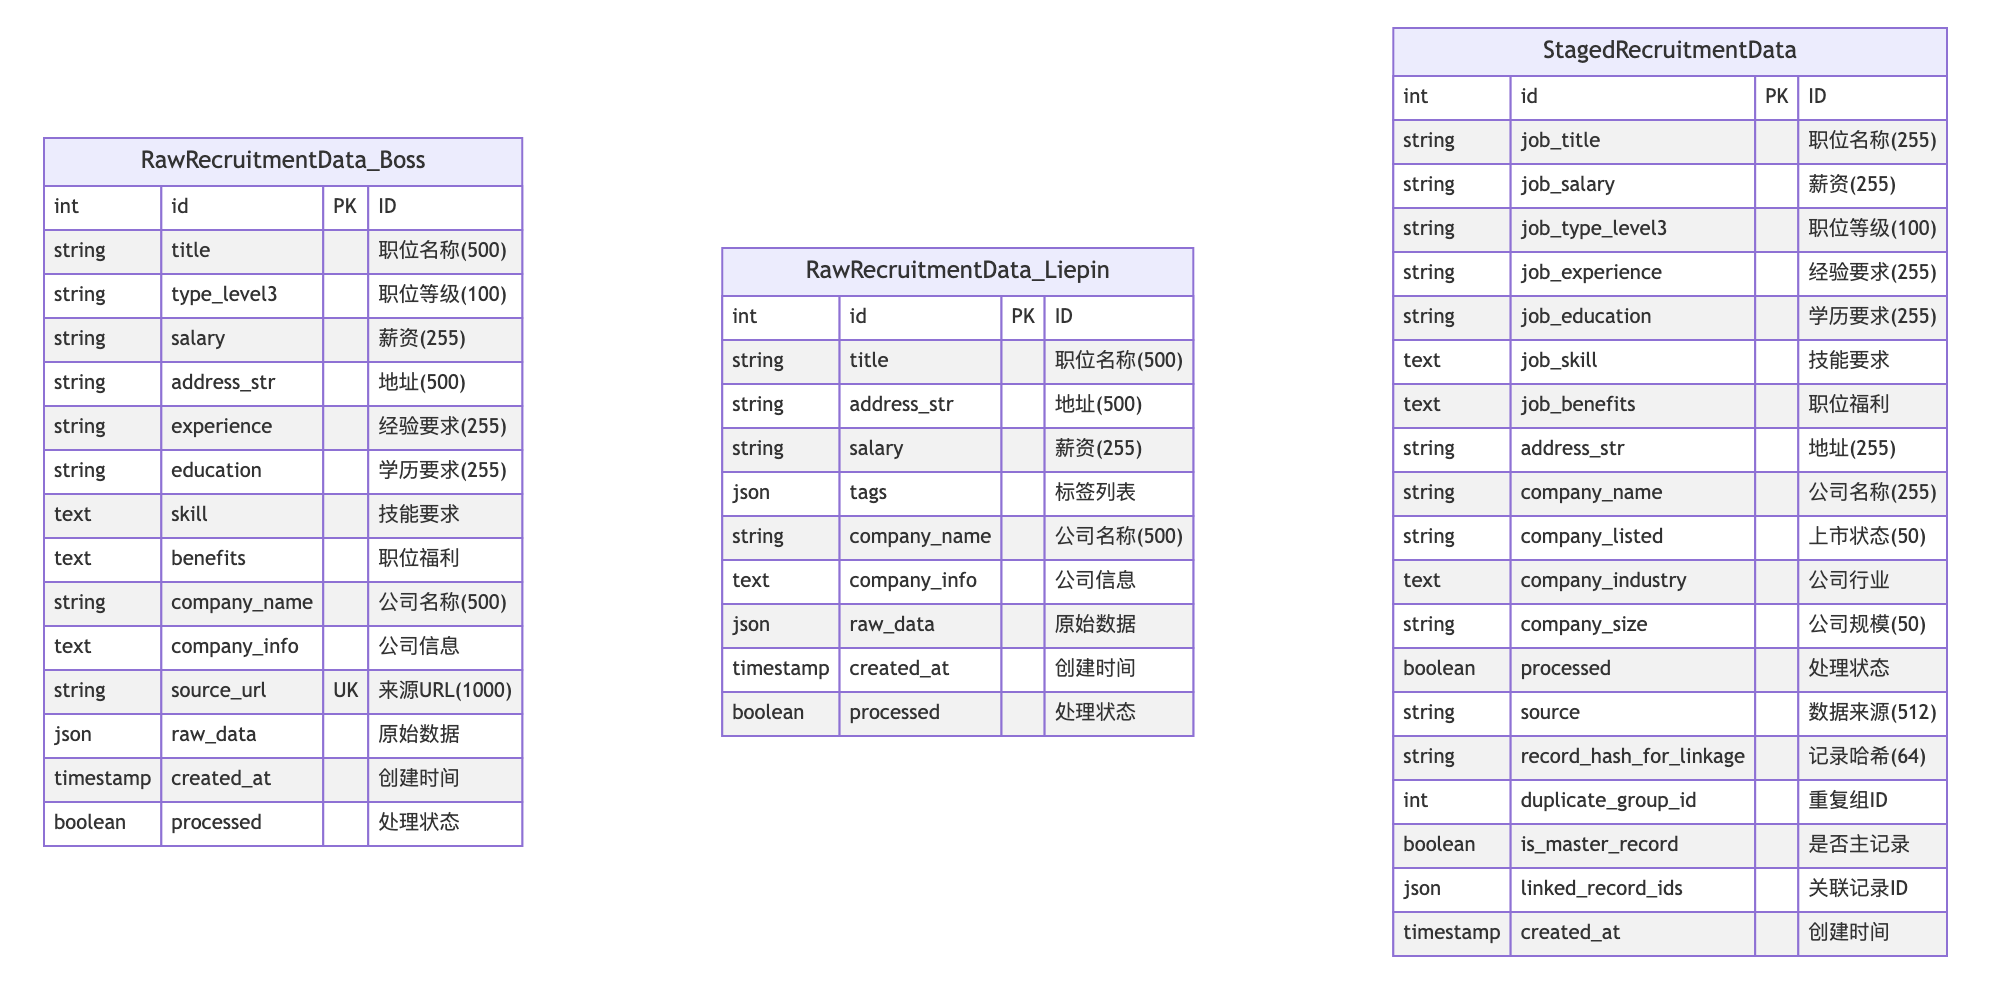
\includegraphics[width=0.8\textwidth]{figures/数据处理层ER图.png}
  \caption{数据处理层E-R图}
  \label{fig:processing_er}
\end{figure}

\paragraph{原始数据表设计}
系统包含两个原始数据表,分别对应不同的数据来源:

\begin{table}[htbp]
  \centering
  \caption{BOSS直聘原始数据表字段设计}
  \label{tab:raw_boss_data_fields}
  \begin{tabular}{@{}lll@{}}
    \toprule
    \textbf{字段类型} & \textbf{字段名} & \textbf{说明} \\
    \midrule
    \multirow{3}{*}{基础信息}
    & id & 主键 \\
    & created\_at & 创建时间 \\
    & processed & 处理状态标记 \\
    \midrule
    \multirow{7}{*}{职位信息}
    & job\_title & 职位名称(500字符) \\
    & job\_level & 职位等级(100字符) \\
    & salary & 薪资(255字符) \\
    & experience & 经验要求(255字符) \\
    & education & 学历要求(255字符) \\
    & skills & 技能要求(文本) \\
    & benefits & 职位福利(文本) \\
    \midrule
    \multirow{2}{*}{公司信息}
    & company\_name & 公司名称(500字符) \\
    & company\_detail & 公司详细信息(文本) \\
    \midrule
    \multirow{3}{*}{其他信息}
    & address & 地址文本(500字符) \\
    & source\_url & 来源URL(1000字符,唯一约束) \\
    & raw\_data & 原始数据(JSON) \\
    \bottomrule
  \end{tabular}
\end{table}

\begin{table}[htbp]
  \centering
  \caption{猎聘网原始数据表字段设计}
  \label{tab:raw_liepin_data_fields}
  \begin{tabular}{@{}lll@{}}
    \toprule
    \textbf{字段类型} & \textbf{字段名} & \textbf{说明} \\
    \midrule
    \multirow{3}{*}{基础信息}
    & id & 主键 \\
    & created\_at & 创建时间 \\
    & processed & 处理状态标记 \\
    \midrule
    \multirow{2}{*}{职位信息}
    & job\_title & 职位名称(500字符) \\
    & salary & 薪资(255字符) \\
    \midrule
    \multirow{2}{*}{公司信息}
    & company\_name & 公司名称(500字符) \\
    & company\_detail & 公司详细信息(文本) \\
    \midrule
    \multirow{3}{*}{其他信息}
    & address & 地址文本(500字符) \\
    & tags & 标签列表(JSON) \\
    & raw\_data & 原始数据(JSON) \\
    \bottomrule
  \end{tabular}
\end{table}

\paragraph{暂存数据表设计}
暂存数据表(StagedRecruitmentData)作为数据清洗和转换的中间层:

\begin{table}[htbp]
  \centering
  \caption{暂存数据表字段设计}
  \label{tab:staged_recruitment_data_fields}
  \begin{tabular}{@{}lll@{}} 
    \toprule
    \textbf{字段类型} & \textbf{字段名} & \textbf{说明} \\ 
    \midrule
    \multirow{7}{*}{职位相关字段} 
    & job\_title & 职位名称(255字符) \\
    & job\_salary & 薪资描述(255字符) \\
    & job\_type\_level3 & 职位等级(100字符) \\
    & job\_experience & 经验要求(255字符) \\
    & job\_education & 学历要求(255字符) \\
    & job\_skill & 技能要求(文本) \\
    & job\_benefits & 职位福利(文本) \\
    \midrule
    \multirow{4}{*}{公司相关字段}
    & company\_name & 公司名称(255字符) \\
    & company\_listed & 上市状态(50字符) \\
    & company\_industry & 公司行业(文本) \\
    & company\_size & 公司规模(50字符) \\
    \midrule
    \multirow{6}{*}{数据处理相关字段}
    & processed & 处理状态标记(布尔值) \\
    & source & 数据来源标识(512字符) \\
    & record\_hash\_for\_linkage & 记录哈希值(64字符),用于快速判断重复 \\
    & duplicate\_group\_id & 重复记录组ID \\
    & is\_master\_record & 主记录标记(布尔值) \\
    & linked\_record\_ids & 关联记录ID列表(JSON) \\
    \bottomrule
  \end{tabular}
\end{table}

\paragraph{数据流转关系}
数据处理层的实体之间形成了清晰的数据流转路径:

\begin{itemize}
    \item 数据采集阶段:
    \begin{itemize}
        \item 爬虫程序分别从BOSS直聘和猎聘网采集数据
        \item 原始数据分别存入对应的原始数据表
        \item 通过processed字段标记数据的处理状态
    \end{itemize}
    
    \item 数据清洗阶段:
    \begin{itemize}
        \item 原始数据经过清洗后存入暂存数据表
        \item 统一数据格式,规范字段命名
        \item 进行数据去重和关联处理
    \end{itemize}
    
    \item 数据转换阶段:
    \begin{itemize}
        \item 暂存数据经过规范化处理
        \item 通过record\_hash\_for\_linkage进行重复检查
        \item 使用duplicate\_group\_id管理重复记录组
        \item 通过is\_master\_record标记主记录
    \end{itemize}
\end{itemize}

这种分层的数据处理设计确保了数据的可追溯性和处理过程的可控性,同时通过合理的字段设计,保证了数据处理的效率和准确性。
\subsection{设计说明}

\subsubsection{分层架构设计说明}

数据库采用分层架构设计,分为数据处理层和规范化数据层。这种分层设计有效分离了数据采集处理和业务数据存储的职责,使系统具有更好的可维护性和扩展性。

\paragraph{数据处理层}
数据处理层不严格遵循第三范式,保留适度的数据冗余以支持数据处理和追溯。该层包含原始数据表和暂存数据表两类重要组件。原始数据表分别存储来自BOSS直聘和猎聘网的爬虫采集数据,完整保留了JSON格式的原始数据,并通过processed字段标记处理状态,支持数据的增量处理和历史追溯。

暂存数据表则作为数据集成的中间层,承担着数据规范化的重要职责。它通过统一的字段命名和格式规范,实现了不同来源数据的模式对齐。同时,暂存表还包含了一系列特殊设计字段,如record\_hash\_for\_linkage和duplicate\_group\_id用于数据去重,is\_master\_record和linked\_record\_ids用于关联记录管理,这些设计为后续的记录链接和数据融合提供了基础支持。

\paragraph{规范化数据层}
规范化数据层严格遵循第三范式设计原则,通过消除数据冗余来保证数据一致性。该层主要由基础实体表、关联关系表和物化视图三部分构成。基础实体表包括用户、公司、职位和地址四个核心实体,每个实体表都独立管理其特有属性。关联关系表(company\_address和job\_address)则专门处理实体间的多对多关系,通过外键约束确保数据完整性。

为了平衡规范化设计带来的查询性能影响,该层还包含了物化视图组件。物化视图通过预先计算和存储常用查询结果,在保证数据一致性的同时提供了优秀的查询性能。这种设计既保持了规范化的优势,又解决了实际应用中的性能需求。

两个数据层之间通过明确的数据流向连接:原始数据经过清洗和转换进入暂存表,再经过规范化处理后存入实体表和关系表,最后通过物化视图提供高效的数据服务。这种渐进式的数据处理流程,确保了数据质量的同时,也保证了整个过程的可控性和可追溯性。
